%%%%%%%%%%%%%%%%%%%%%%%%%%%%%%%%%%%%%%%%%
% Beamer Presentation
% LaTeX Template
% Version 1.0 (10/11/12)
%
% This template has been downloaded from:
% http://www.LaTeXTemplates.com
%
% License:
% CC BY-NC-SA 3.0 (http://creativecommons.org/licenses/by-nc-sa/3.0/)
%
%%%%%%%%%%%%%%%%%%%%%%%%%%%%%%%%%%%%%%%%%

%----------------------------------------------------------------------------------------
%	PACKAGES AND THEMES
%----------------------------------------------------------------------------------------

\documentclass[aspectratio=149]{beamer}
\usefonttheme[onlymath]{serif}


\mode<presentation> {

% The Beamer class comes with a number of default slide themes
% which change the colors and layouts of slides. Below this is a list
% of all the themes, uncomment each in turn to see what they look like.

\usetheme{default}
%\usetheme{AnnArbor}
%\usetheme{Antibes}
%\usetheme{Bergen}
%\usetheme{Berkeley}
%\usetheme{Berlin}
%\usetheme{Boadilla}
%\usetheme{CambridgeUS}
%\usetheme{Copenhagen}
%\usetheme{Darmstadt}
%\usetheme{Dresden}
%\usetheme{Frankfurt}
%\usetheme{Goettingen}
%\usetheme{Hannover}
%\usetheme{Ilmenau}
%\usetheme{JuanLesPins}
%\usetheme{Luebeck}
%\usetheme{Malmoe}
%\usetheme{Marburg}
%\usetheme{Montpellier}
%\usetheme{PaloAlto}
%\usetheme{Pittsburgh}
%\usetheme{Rochester}
%\usetheme{Singapore}
%\usetheme{Szeged}
%\usetheme{Warsaw}

% As well as themes, the Beamer class has a number of color themes
% for any slide theme. Uncomment each of these in turn to see how it
% changes the colors of your current slide theme.

%\usecolortheme{albatross}
\usecolortheme{beaver}
%\usecolortheme{beetle}
%\usecolortheme{crane}
%\usecolortheme{dolphin}
%\usecolortheme{dove}
%\usecolortheme{fly}
%\usecolortheme{lily}
%\usecolortheme{orchid}
%\usecolortheme{rose}
%\usecolortheme{seagull}
%\usecolortheme{seahorse}
%\usecolortheme{whale}
%\usecolortheme{wolverine}

%\setbeamertemplate{footline} % To remove the footer line in all slides uncomment this line
%\setbeamertemplate{footline}[page number] % To replace the footer line in all slides with a simple slide count uncomment this line

%\setbeamertemplate{navigation symbols}{} % To remove the navigation symbols from the bottom of all slides uncomment this line
}

\usepackage{graphicx} % Allows including images
\usepackage{booktabs} % Allows the use of \toprule, \midrule and \bottomrule in tables
\usepackage{verbatim}

\usepackage{mathtools} 
\usepackage{amssymb}
\usepackage{mathrsfs}
\usepackage{amsmath}

\usepackage{ragged2e}
\usepackage{etoolbox}
\usepackage{lipsum}

\usepackage{siunitx,booktabs}
\usepackage{pifont}




\setbeamertemplate{enumerate items}[circle]
\usepackage{tikz}

\newcommand\mynum[1]{
  \usebeamercolor{enumerate item}
  \tikzset{beameritem/.style={circle,inner sep=0,minimum size=2ex,text=enumerate item.bg,fill=enumerate item.fg,font=\footnotesize}}%
  \tikz[baseline=(n.base)]\node(n)[beameritem]{#1};
}

\newcommand\mynumm[1]{
  \usebeamercolor{enumerate item}
  \tikzset{beameritem/.style={rectangle,inner sep=0,minimum size=2ex,text=enumerate item.bg,fill=enumerate item.fg,font=\footnotesize}}%
  \tikz[baseline=(n.base)]\node(n)[beameritem]{#1};
}

\def\Put(#1,#2)#3{\leavevmode\makebox(0,0){\put(#1,#2){#3}}}

\newcommand\Wider[2][3em]{%
\makebox[\linewidth][c]{%
  \begin{minipage}{\dimexpr\textwidth+#1\relax}
  \raggedright#2
  \end{minipage}%
  }%
}

\setbeamertemplate{footline}[frame number]

%----------------------------------------------------------------------------------------
%	TITLE PAGE
%----------------------------------------------------------------------------------------

\title{ Microcredit from Delayed Bill Payments } % The short title appears at the bottom of every slide, the full title is only on the title page

\author{Will Violette} 

 % Your institution as it will appear on the bottom of every slide, may be shorthand to save space

\date{\footnotesize The views expressed herein do not necessarily reflect those of the Federal Trade Commission or any of its commissioners.} % Date, can be changed to a custom date
%\today

\begin{document}

\beamertemplatenavigationsymbolsempty

\begin{frame}
\titlepage % Print the title page as the first slide
\end{frame}

%\begin{frame}
%\frametitle{Overview} % Table of contents slide, comment this block out to remove it
%\tableofcontents % Throughout your presentation, if you choose to use \section{} and \subsection{} commands, these will automatically be printed on this slide as an overview of your presentation
%\end{frame}

%----------------------------------------------------------------------------------------
%	PRESENTATION SLIDES
%----------------------------------------------------------------------------------------
\section{Introduction}
%------------------------------------------------

% \begin{frame}
% \frametitle{ Motivation }

% \begin{itemize}
% \item Households experience large month-to-month changes in income
% \begin{itemize}
%   \item Coef. of variation $\sim$0.4 in US and Mexico \\ {\scriptsize (Hannagan and Morduch [2015]; Amuedo-Dorantes and Pozo [2011]) }
% \end{itemize}

% \vspace{2mm}

% \item Short-term credit to smooth consumption is costly 
%   \begin{itemize}
%     \item High interest rates from payday loans, credit cards, informal moneylenders, etc.
%     \item In Manila, only 4\% have credit cards, 19\% have bank accounts
%   \end{itemize}
% \end{itemize}
% \end{frame}


\begin{frame}
\frametitle{ Motivation }


\begin{itemize}
\item Households (HHs) have variable, uncertain incomes
\vspace{2mm}
\item Smoothing consumption is costly 
  \begin{itemize}
    \item High interest rates from payday loans, credit cards, informal moneylenders, etc.
    \item In Manila, only 4\% have credit cards, 19\% have bank accounts
  \end{itemize}

\vspace{2mm}

\item Public utilities (water, electricity, gas, etc.) may provide efficient, second-best credit by letting HHs delay their bill payments
  \vspace{1mm}

  % \begin{enumerate}
  %   \item \textbf{Collateral} from disconnections for nonpayment
  %    \vspace{1mm}
  %   \item \textbf{Low monitoring costs} since workers already service connections
  %    \vspace{1mm}
  %   \item \textbf{Wide risk pool} due to nearly universal coverage 
  %    \vspace{1mm}
  %   \item \textbf{Few consumption distortions} due to inelastic demand for utilities
  % \end{enumerate}
\end{itemize}

\end{frame}

%------------------------------------------------

\begin{frame}
\frametitle{ New policies reduce delinquency }


\begin{itemize}
  \item Growing use of prepaid meters that ensure upfront payments
  \vspace{.1cm}
  \begin{itemize}
    \item benefits $\rightarrow$ may lower prices and increase investments in quality
    \item costs $\rightarrow$ no more credit from delayed bill payments
  \end{itemize}
\begin{figure}
\centering
\caption{Prepaid water meter in South Africa}
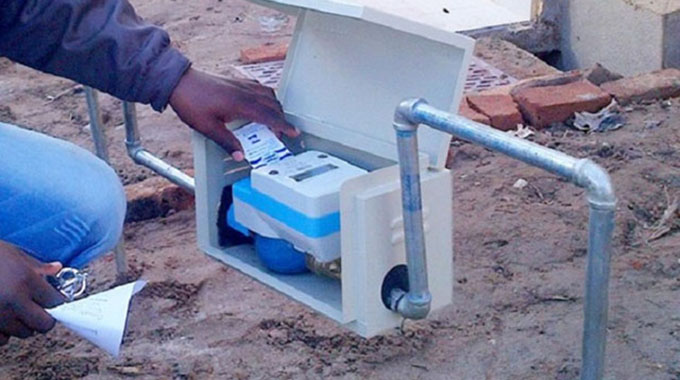
\includegraphics[scale=.2]{prepaid-water-meter.jpg}
\end{figure}
\end{itemize}

\begin{itemize}
\item \textbf{Research Question} \hspace{.5mm} how much do HHs value delaying their bills?
\vspace{.1cm}
\begin{itemize}
  \item How credit-constrained are HHs?
  \item What are the welfare effects of other payment policies \\ (ie. prepaid meters)?
\end{itemize}
\end{itemize}
% \begin{itemize}
%   \item In the US, states often encourage utility credit by limiting disconnections for delinquency
%     \vspace{1mm}
%     \begin{itemize}
%       \item Often cite health reasons {\footnotesize (Focus for future research, LIHEAP [2019]))}
%     \end{itemize}
% \end{itemize}



\end{frame}

%------------------------------------------------

\begin{frame}
\frametitle{This Paper}

\begin{itemize}
% \item \textbf{Question} \hspace{.5mm} how much do HHs value delaying their bills?
% \vspace{.1cm}
% \begin{itemize}
%   \item How credit-constrained are HHs?
%   \item What are the welfare effects of other payment policies \\ (ie. prepaid meters)?
% \end{itemize}
\vspace{2mm}
\item \textbf{Context} \hspace{.5mm} a regulated piped water utility in Manila
\vspace{2mm}
\item \textbf{Data} \hspace{.5mm} monthly billing records from 2010-15 for 1.5 mil. connections
\vspace{2mm}
\item \textbf{Approach} \hspace{.5mm} estimate a consumption/savings model where HHs choose when to pay their water bills
% \vspace{1mm}
% \begin{itemize}
%   \item Estimate credit constraints from billing delinquency
%   \item Simulate counterfactuals
% \end{itemize}
\vspace{2mm}
\item \textbf{Results} \hspace{.5mm} monthly interest rate is 2.2\%  (30\% annually) and willingness-to-pay for delaying bills is 70 PhP (or \$1.5) per month 

  
\begin{itemize}

  \item Prepaid metering (adjusting prices to cover costs) reduces welfare

\end{itemize}


\end{itemize}

\end{frame}

%------------------------------------------------
%------------------------------------------------

% \begin{frame}
% \frametitle{Preview of Results}

% \begin{itemize}
%   \item Estimated monthly interest rate is 2.2\%  (30\% annually)
%   \vspace{1mm}
%     \begin{itemize}
%       % \item In Manila, moneylenders offer 20\% monthly { \footnotesize (Karlan and Zinman [2009])}
%       %   \vspace{1mm}
%       \item Globally, microfinance offers 13 to 25\% annually { \footnotesize (Cull et al. [2009])}
%     \end{itemize}

% \vspace{2mm}

%   \item Willingness-to-pay for delaying bills is $\sim$70 PhP (or \$1.5) per month 
%   \vspace{1mm}
%   \begin{itemize}
%     \item Equal to 9\% of an avg water bill
%     % and 0.2\% of HH income
%   \end{itemize}

% \vspace{2mm}

%   \item Prepaid metering (adjusting prices to cover costs) reduces welfare

% \end{itemize}

% \end{frame}

% monthly = ((1+annual)^(1/12)) - 1
% annual = ((monthly + 1)^(12)) - 1

%------------------------------------------------
%------------------------------------------------


\begin{frame}
\frametitle{Contributions to the Literature}

\begin{enumerate}
\item Bring consumption smoothing to public utility regulation \\
{\footnotesize (McRae [2015]; Szab\'o [2015]; Jack and Smith [2015,2016]; Szab\'o and Ujhelyi [2015])}
\vspace{2mm}

\item Estimate HH consumption/savings model with utility billing data \\
{\footnotesize (Deaton [1991]; Gourinchas and Parker [2002]; Laibson et al. [2007])}
\vspace{2mm}

\item Measure credit constraints from billing delinquency \\
{ \footnotesize (\textit{RCTs}: Karlan and Zinman [2009]; Gin\'e and Karlan [2014],  \textit{Village surveys}: Townsend [1994]; Townsend and Kinnan [2012]; Ligon [1994], \textit{Natural Experiments}: Banerjee and Duflo [2012]) }

\end{enumerate}

\end{frame}



%------------------------------------------------
%------------------------------------------------

\begin{frame}
\frametitle{Model of HH consumption and savings}

% u(w_{\tau},x_{\tau})
\begin{align*}\label{eq:u}
&max \, \, \, E_t \Big[ \, \, \sum_{\tau = t}^{\infty} (1+\delta)^{t-\tau} \,\, u(w_{\tau},x_{\tau}) \, \, \Big] \\
\forall t &\,\,\,\,\,x_t \, + \, p(w_t) w_t \, = \, y_t \, + A_t - \frac{ A_{t+1} }{1+r_a} + S_t
\end{align*}

\begin{itemize}
\item Utility, $u(w_{\tau},x_{\tau}) =\alpha log( w_{\tau}) + (1-\alpha) log(x_{\tau})$ is over water, $w_t$, and all other goods, $x_t$, with discount rate, $\delta$
\vspace{.5mm}
\item Budget constraint has water price, $p(w_t)$, and income, $y_t$, which takes values $(1+\theta)\bar{y}$ and $(1-\theta)\bar{y}$ with 0.5 probability
\vspace{.5mm}
\item HHs borrow and save with asset $A_{t+1}$ where $A_{t+1}\geq -\bar{A}$ and interest rate, $r_a$, is  equal to $r_h$ if borrowing ($A_{t+1}\leq 0$) and $r_l$ else
\vspace{.5mm}
\item $S_t$ allows for borrowing from water bills (cont.)
\end{itemize}

\end{frame}


\begin{frame}
\frametitle{Borrowing from water bills, $S_t$}

\begin{itemize}
\item Each period, HH faces probability $\pi$ of receiving a delinquency visit from the water utility
\item If no visit occurs, HHs can borrow by not paying their bills
\begin{align*}
S_t &= B_{t-1} -  B_{t} \\
B_{t-1} &-  p(w_t) w_t \leq B_{t} \leq 0 
\end{align*}

\begin{itemize}
  \item $B_{t-1}$ : last month's unpaid bill { \footnotesize ($\leq0$) }
  \item $B_{t}$ : this month's unpaid bill { \footnotesize ($=0$ if $A_t>0$ to prevent arbitrage)}
  % \item $r_{b}$ : bill interest rate (equal to $r_h$ if $A_t>0$ to prevent arbitrage)
  % \item HHs can borrow up to their unpaid bills plus their current usage
\end{itemize}
\vspace{2mm}


\item If a visit occurs, HHs can choose to disconnect ($D_{t}=1$), avoid paying their bills ($S_t  = 0$), and pay a fixed cost ($f$) per month for other water until they reconnect

\item Otherwise, HHs pay off any unpaid bills ($S_t=B_{t-1}$) and this month's bill ($B_{t}=0$) to stay connected

\end{itemize}

\end{frame}






%------------------------------------------------

%------------------------------------------------

\begin{frame}
\frametitle{Data and Sample}

\begin{itemize}
  \item Data
    \begin{itemize}
      \item Monthly billing records per connection 2010-15 \\
      (usage, payments, and delinquency visits)
      \vspace{2mm}
      \item Merge to survey data on $\sim$50,000 connections \\
      (number of HHs sharing a connection and demographics for the owner)
    \end{itemize}
    \vspace{2mm}
  \item Sample
    \begin{itemize}
      \item Model single HH decisions
        \begin{itemize}
          \item Keep residential connections that serve a single HH (67\%) 
          \vspace{1mm}
        \end{itemize}
      \item Use delinquency visits for identification
        \begin{itemize}
          \item Keep HHs with visits (31\%) 
        \end{itemize}
         \vspace{1mm}
      \item Drop HHs that move
        \begin{itemize}
          \item Drop if disconnected for the last 6 months of the sample (10\%) 
        \end{itemize}
    \end{itemize}
\end{itemize}

\end{frame}

%------------------------------------------------

\begin{frame}
\frametitle{Descriptives}

% \Wider{
% \begin{table}[H]
% \centering
% %\caption{Descriptives}\label{table:descriptives_stayers}
% \vspace{-2mm}
% % \resizebox{1.05\linewidth}{!}{
% \begin{tabular}{l*{1}{cccccc}}
% \toprule
%  & Mean & SD & Min & 25th & 75th & Max  \\
% \midrule
%  Usage (m3)  & 30.0  & 20.5  & 0.0  & 17.0  & 38.0  & 200.0  \\ 
 Bill  & 931  & 1,269  & -4,862  & 323  & 1,122  & 78,409  \\ 
 Unpaid Balance  & 3,009  & 5,953  & -4,995  & 330  & 3,016  & 79,959  \\ 
 Share of Months with Payment  & 0.62  & 0.49  & 0.00  & 0.00  & 1.00  & 1.00  \\ 
 Payment Size  & 1,448  & 1,769  & 0  & 500  & 1,753  & 76,029  \\ 
 Days Delinquent  & 90.9  & 161.8  & 0.0  & 0.0  & 91.0  & 720.0  \\ 
 Delinquency Visits per HH  & 1.35  & 0.63  & 1.00  & 1.00  & 2.00  & 6.00  \\ 
 Share of Months Disconnected  & 0.04  & 0.19  & 0.00  & 0.00  & 0.00  & 1.00  \\ 

% \bottomrule
% \multicolumn{7}{c}{Total Households: 11,856  Obs. per Household: 61.8 Total Obs.: 731,935}
% \end{tabular}
% %}
% \end{table}
% }

% \begin{table}[H]
% \centering
% \vspace{-2mm}
% \begin{tabular}{l*{1}{cc}}
% % \toprule
%  & Mean & SD  \\
% \midrule
%  Usage (m3)  & 26.2  & 17.5  \\ 
 Bill  & 761  & 1,124  \\ 
 Unpaid Balance  & 2,416  & 5,070  \\ 
 Share of Months with Payment  & 0.60  & 0.49  \\ 
 Days Delinquent  & 84.9  & 155.4  \\ 
 Delinquency Visits per HH  & 1.32  & 0.61  \\ 
 Share of Months Disconnected  & 0.03  & 0.17  \\ 

% % \bottomrule
% \end{tabular}
% % }
% \end{table}

\begin{itemize}
\item Avg water bill is 761 PhP while avg unpaid balance is 2,416 PhP ($\sim$5\% of HH income)
\vspace{.8mm}
\item HHs pay in 60\% of months
\vspace{.8mm}
\item There are 1.32 delinquency visits per HH on avg
\vspace{.8mm}
\item Sample has 11,856HHs with 61.8obs per HH for 731,935total obs 
\end{itemize}

\vspace{3mm}
45 Philippine Peso (PhP) = 1 US Dollar \\
Avg monthly HH Income 31,910PhP \\
% \begin{itemize}
% \item Why do households pay late? (convenience, consumption smoothing)
% \end{itemize}

\end{frame}


%------------------------------------------------
%------------------------------------------------

\begin{frame}
\frametitle{Avg share connected around 1st delinquency visit}
\Wider[4em]{
\begin{figure}
\centering
%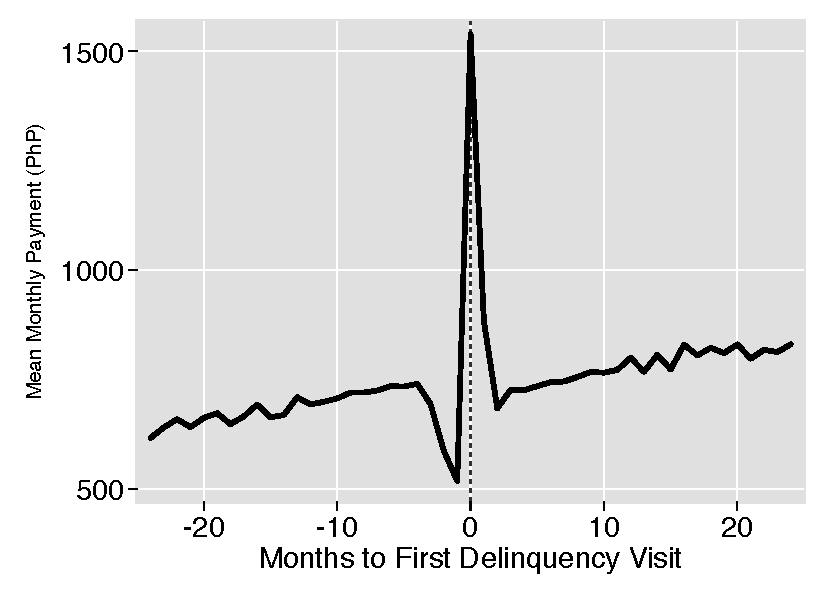
\includegraphics[scale=.47]{tables/line1_pay.pdf}
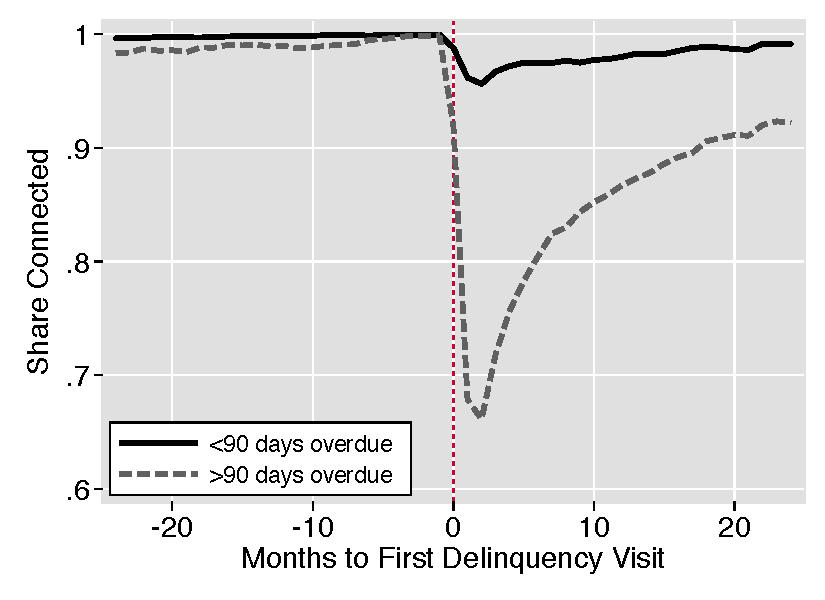
\includegraphics[scale=.7]{tables/line_conn.pdf}
\end{figure}
}
\end{frame}


%------------------------------------------------
%------------------------------------------------


\begin{frame}

\frametitle{Estimates with simulated method of moments}
\Wider[4em]{

\begin{table}[H]
\centering
% \caption{Calibrated and Assumed Parameters}\label{table:calibratedparam}
\begin{tabular}{l*{1}{lll}}
%\toprule
%Parameter  &   &  Value & Source \\
%\midrule
Calibrated & & & Source \\[.5em]
%\toprule
Discount rate  & $\delta$ & 0.015 & {\footnotesize Structural macro literature} \\
Savings rate & $r_l$ & 0.003 & {\footnotesize World Bank} \\
 Visit risk & $\pi$ & 0.04 & {\footnotesize Billing data }  \\
Price  & $p$ & 20.2 + 0.2w & {\footnotesize Billing data } \\
Mean inc. (PhP) & $\bar{y}$ & 31,910 & {\footnotesize HH inc. survey} \\
Borrowing limit & $\bar{A}$ & -32,250 & {\footnotesize HH inc. survey (95 pctile. of loans)} \\
Unpaid bills limit & $\bar{B}$ & -10,109 & {\footnotesize Billing data (95 pctile. of unpaid bills)} \\
%\bottomrule 
\\
Estimated  &  & & Moments\\[.5em]
%\toprule
Water preference & $\alpha $ &0.025
 (0.00013
\unskip)  & {\footnotesize   Avg usage   } \\[.1em]
Income shock size  & $\theta $ &  0.342
 (0.0318
\unskip)  & {\footnotesize  Avg unpaid bills } \\[.1em]
Cost of other water  &  $f$ & 198.9
 (34.3\unskip) &  {\footnotesize  \% Disc. 1-2 months post visit } \\[.1em]
Borrowing rate & $r_h$ & 0.022
  (0.0011
\unskip)    & \% {\footnotesize  Disc. 1-2 months post visit } \\
% & &   %  {\footnotesize \hspace{4mm} given $>$90 days overdue} \\

% \end{tabular}
% \begin{tabular}{l*{1}{l}}

% \textbf{To be estimated}  & & \textbf{Identifying moments}\\[.5em]
% %\multicolumn{3}{l}{\scriptsize All measures are monthly. } \\[-.5em]
% Water preference & $\alpha $ & {\footnotesize   Avg usage   } \\[.1em]
% Income shock size  & $\theta $ & {\footnotesize  Avg unpaid bills } \\[.1em]
% Cost of other water  &  $f$ & {\footnotesize  \% Disc. 1-2 months post visit } \\[.1em]
% Borrowing rate & $r_h$ & \% {\footnotesize  Disc. 1-2 months post visit } \\
%  & &  {\footnotesize \hspace{4mm} given $>$90 days overdue} \\
\end{tabular}
\end{table}
}
%{\footnotesize All terms are monthly}

\end{frame}





% \begin{frame}

% \frametitle{Estimation with simulated method of moments}

% \begin{table}[H]
% \centering
% % \caption{Calibrated and Assumed Parameters}\label{table:calibratedparam}
% \begin{tabular}{l*{1}{ll}}
% Estimated Parameters  & & Moments \\[.5em]
% \toprule
% %\multicolumn{3}{l}{\scriptsize All measures are monthly. } \\[-.5em]
% Water preference & $\alpha $ & {\footnotesize   Avg usage   } \\[.1em]
% Income shock size  & $\theta $ & {\footnotesize  Avg unpaid bills } \\[.1em]
% Fixed cost of other water  &  $f$ & {\footnotesize  \% Disc. 1-2 months post visit } \\[.1em]
% Borrowing rate from standard assets & $r_h$ & \% {\footnotesize  Disc. 1-2 months post visit } \\
%  & &  {\footnotesize \hspace{4mm} given $>$90 days overdue} \\
% \end{tabular}
% \end{table}

% \begin{itemize}
% \item Solve for the optimum of a grid of 28 asset and 28 billing values
% \item Compute simulated moments (avg usage, unpaid bills, etc.) with a random sequence of 10,000 states
% \item Choose parameters to minimize the sum of squared distances between the data and the simulated moments
% \end{itemize}

% \end{frame}


% \begin{frame}
% \frametitle{Estimates}

% \begin{table}[h!]
% \centering
% %\caption{Estimates}\label{table:estimates}
% \vspace{-2mm}
% %\resizebox{\columnwidth}{!}{%
% \begin{tabular}{l*{1}{cc}}
% %\toprule
% Parameters  &   & Estimates \\
% \midrule
% Water Preference & $\alpha$ & 0.025
 \\
%  &  & (0.00013
\unskip) \\[.4em]
% Income shock size & $\theta$ & 0.342
 \\
%  &  & (0.0318
\unskip) \\[.4em]
% Fixed cost of other water (PhP) & $f$ &  198.9
 \\
%  &  &  (0.0
\unskip) \\[.4em]
% Borrowing rate from standard assets & $r_h$ & 0.022
 \\
%  &  & (0.0011
\unskip) \\[.8em]
% Households & & 11,856 \\
% Household-Months & & 731,935 \\
% \bottomrule
% \multicolumn{3}{l}{\scriptsize Standard errors in parentheses are bootstrapped at the household-level.} % with 4
repetitions 
% \end{tabular}
% %}
% \end{table}

% \end{frame}


\begin{frame}
\frametitle{Counterfactuals}

\Wider[4em] { %%%% widen the whole thing!

\begin{table}[H]
\centering
%\caption{Counterfactual Policies}\label{table:counter}
\resizebox{\columnwidth}{!}{%
\begin{tabular}{lcc<{\onslide<2->}c<{\onslide<3->}c<{\onslide}}
\toprule
 & (1) & (2) & (3) & (4) \\
 & Current & No Water   & No Water Borrowing    & Prepaid Metering \\
 &         & Borrowing  & and Covering Costs      & and Covering Costs   \\
\midrule   
Compensating Variation (PhP) &  & -69.3
 & -33.2
  & -225.2
 \\
Mean Usage (m3) & 26.58
 & 24.22
  & 24.18
 & 21.54
 \\[.2em]
 &         &           &         &  \\
% Water Borrowing  & \checkmark & X & X & X \\[.2em]
%Adjustments to stay revenue neutral  & & \\
\onslide<2-> Price Intercept (PhP/m3) & 20.23
 &   &  20.27
 & 26.63
 \\[.2em]
\onslide<2->  Credit supply costs (PhP) & 31.3 &   & 0 & 0 \\[.2em]
% \onslide<2-> Disconnection Rebate (PhP) & 10.2 &   & 0 & 0 \\[.2em]
% \onslide<2-> Delinquency Visit Cost (PhP) & 6.3
 &  & 0 & 0 \\[.2em]
% \onslide<2-> Opp. Cost of Lending (PhP) & 41.5
 &  & 0 & 0 \\[.2em]

\onslide<2-> Marginal cost (PhP/m3) & 5 &   & 5 & 5 \\[.2em]
\onslide<3-> Additional metering cost (PhP) &  0 &  & \onslide<3-> 0 & 51 \\[.2em]
%Price Intercept (PhP)  &20.2& &26.6\\

%Fixed Savings (PhP)  &19.1& &0\\

\bottomrule
\multicolumn{5}{l}{  All values are at the household-month level. }
%The price intercept increases under prepaid metering to cover meter replacement } % \\[-.5em]
%\multicolumn{5}{l}{ \scriptsize  costs.  The disconnection rebate measures the average outstanding balance left unpaid by permanently disconnected households } \\[-.5em]
%\multicolumn{5}{l}{ \scriptsize  in terms of household-months.  Price intercepts and disconnection rebates are unchanged for the no water } \\[-.5em]
%\multicolumn{5}{l}{ \scriptsize  borrowing counterfactual.}
\end{tabular}
}
\end{table}

} %%%% widen the whole thing!


\begin{itemize}
 \onslide<2>  \item Credit supply costs include (1) cost of delinquency visits, (2) lost revenue from HHs that move, and (3) opportunity cost of credit
\end{itemize}

\end{frame}



\begin{frame}

% \frametitle{Next Steps}

% \begin{itemize}
%   \item Estimate heterogeneity by income
%   \item Model HHs decision to move out of Manila (and leave outstanding bills)
%   \item Optimal delinquency visit policy for Manila
% \end{itemize}
\vspace{2mm}
Thank you!

\end{frame}



\begin{frame}
\frametitle{Other outcomes relative to 1st visit}
\Wider[4em]{
\begin{figure}
\centering
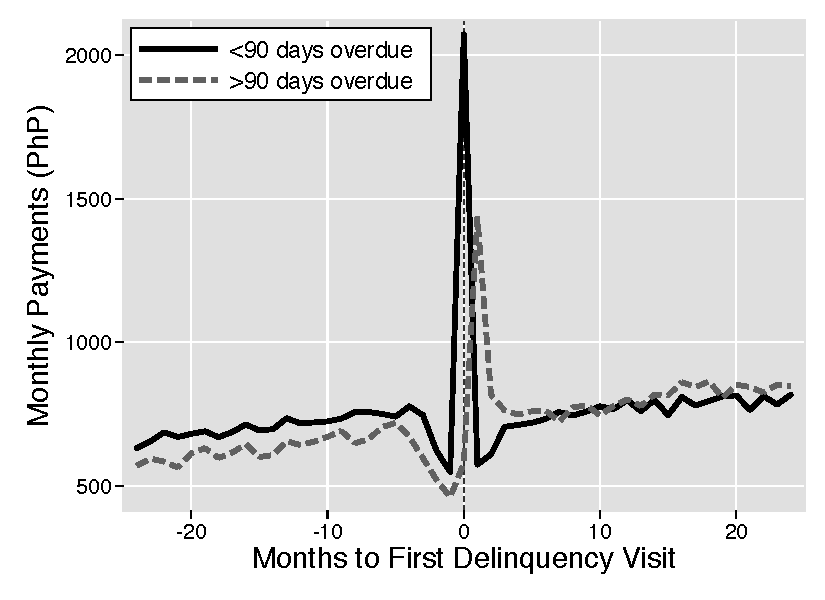
\includegraphics[scale=.47]{tables/line_pay.pdf}
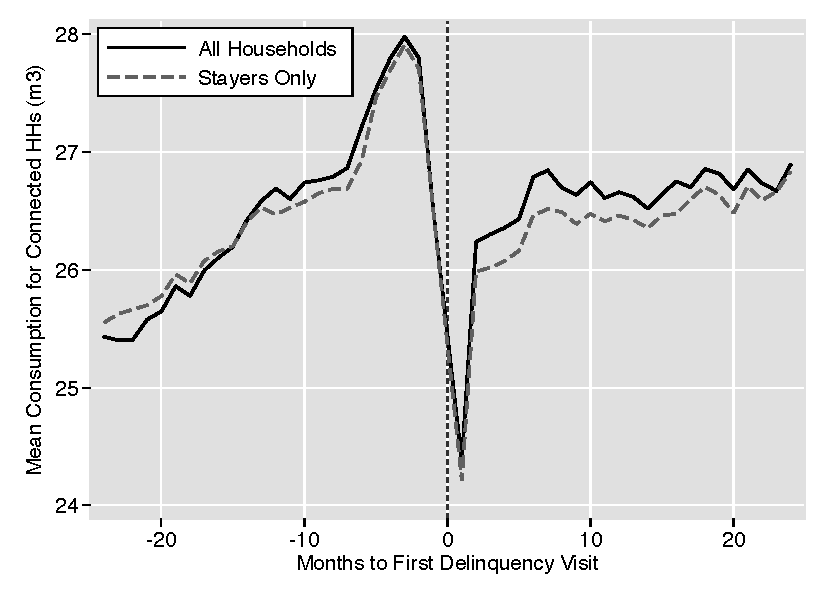
\includegraphics[scale=.47]{tables/line_c.pdf}
\end{figure}
\begin{itemize}
  \item Avg payments only include positive payments
\end{itemize}
}
\end{frame}


%------------------------------------------------
%------------------------------------------------

\begin{frame}
\frametitle{Solving the model with a value function approach}

\begin{align*}
V(X_t,z_t) \,=\, &max_{x_t,w_t}  \,\,\, u(x_t,w_t) \,+\,\, (1+\delta)^{-1} \, E \Big[\, V(X_{t+1}|z_{t})\,\Big| z_{t+1}, T_{t,t+1} \Big]
\\
s.t.& \\
x_t & \, + \, p(w_t) w_t \, = \, y_t  \, + \, S_t \\
B_{t-1}-p&(w_t) w_t (1-D_{t}) \leq B_{t} \leq 0  \\
\\
X_t &= [x_{t},w_{t},A_{t},B_{t},D_{t}] \hspace{2mm}\text{ chosen by HH }  \\
 z_t &= [y_t,visit_t]  \\
T_{t,t+1} &= [ 0.5\pi \,\,\,\, 0.5(1-\pi)\,\,\,\,  0.5\pi\,\,\,\,  0.5(1-\pi) ] \times [ 1 \,\,\,\, 1\,\,\,\,  1 \,\,\,\, 1 ]^{\text{T}}
% \text{simple transition matrix } \\ 
\end{align*}


% \vspace{2mm}
% \begin{itemize}
% \item Choices observed in the data : usage ($w_t$), bills ($B_t$), and disc. ($D_t$)
% \end{itemize}

\end{frame}





%------------------------------------------------

% \begin{frame}
% \frametitle{Paying water bills in Manila}

% \begin{enumerate}
% \item The avg HH is 85 days behind on their payments
%   \begin{itemize}
%     \item Avg HH's unpaid water bills = 5\% monthly HH income
%  %   \item Two main reasons: Inconvenient to pay every month and Consumption smoothing
%   \end{itemize}
% \vspace{3mm}
% \item No interest is charged on delinquent bills 
% % and many options for paying \\
% % { \footnotesize (gas stations, convenient stores, phone, online, or via ATM kiosks) }
% \vspace{3mm}
% % \item After 60 days of delinquency, regulations permit disconnection
% \item The utility visits delinquent HHs and makes a take-it or leave-it offer: \\ pay now or become disconnected % sudden take-it-or-leave-it offer
% \vspace{.5mm}
%   \begin{itemize}
%     \item Visits are rare (4\% of HH-months given $>$60 days delinquent)
%     % \item HHs pay immediately to avoid disconnection
%     % \item Others disconnect until they can afford to reconnect
%   \end{itemize}
% \vspace{3mm}
% \item To reconnect, HHs pay a small one-time fee and all unpaid bills
% \vspace{.5mm}
%   \begin{itemize}
%     \item When HHs change residences, they rarely pay their outstanding bills 
%   \end{itemize}

% \end{enumerate}
% \end{frame}




\end{document} 
